\documentclass[11pt]{article}
\usepackage{acl2016}
\usepackage{times}
\usepackage{latexsym}
\usepackage{graphicx}
\usepackage{url}
\usepackage{subfigure}
\usepackage{pgfplotstable}
\usepackage{hyperref}
\usepackage{color}
\usepackage{lipsum,adjustbox}

\newcommand{\com}[1]{}
\newcommand{\secref}[1]{Section \ref{#1}}
\newcommand{\figref}[1]{Figure~\ref{#1}}
\newcommand{\tabref}[1]{Table~\ref{#1}}
\newcommand{\oa}[1]{\footnote{\color{red} #1}}
\newcommand{\bh}[2]{\footnote{\color{blue} #1}}

\newcommand\BibTeX{B{\sc ib}\TeX}


\title{HUME: Human UCCA-based Machine-Translation Evaluation}

\author{Author 1\\
	    XYZ Company\\
	    111 Anywhere Street\\
	    Mytown, NY 10000, USA\\
	    {\tt author1@xyz.org}
	  \And
	Author 2\\
  	ABC University\\
  	900 Main Street\\
  	Ourcity, PQ, Canada A1A 1T2\\
  {\tt author2@abc.ca}}

\date{}

\begin{document}

\maketitle

\begin{abstract}

  Semantic evaluation of Machine Translation (MT) systems, informative as for
  semantic discrepencies between the translation and the source text,
  has become a necessity, given recent interest in semantics-aware MT systems.
  We present a novel human semantic evaluation measure for MT, Human
  UCCA-based MT evaluation (HUME), building on the UCCA semantic representation scheme.
  Making progress over previous work, the proposed measure takes into account
  a wider range of semantic phenomena and does not rely on semantic annotation
  of the MT output, whose interpretation is often unclear. 
  We experiment with four language pairs, demonstrating the broad applicability of
  the measure, as well as its reliability, reflected by the inter-annotator agreement
  scores.

\end{abstract}


%%%%%%%%%%%%%%%%%%%%%%%%%%%%%%%%%%%%%%%%%%%%%%%%%%%%%%%%%%%%%%%%%%%%%%%%%%%%%%%%%%%%%%
\section{Introduction}\label{sec:intro}

Human judgement is the central, and perhaps ultimate, criterion for estimating the
quality of an MT system.
Nevertheless, common measures for MT evaluation, such as adequacy and frequency judgements
or the relative ranking of several possible translations, are problematic in two ways.
First, as the quality of translation is determined by multiple factors, it is difficult
to assign a single number that quantifies the quality of the entire sentence, as is reflected
by the diminishing inter-annotator agreement rates of human ranking measures
as a function of the sentence length \cite{Bojar:2011}.
Second, a sentence-level quality score does not indicate what parts of the sentence
are erroneously translated in the output, and hence cannot inform developers in overcoming these errors.
This problem can be addressed by using scores that decompose over the sub-parts of the sentence. 
However, common decompositions into n-grams or even individual words, as employed by the
popular BLEU \cite{Papineni:2002} and METEOR measures \cite{Banerjee:2005},
are most suitable for evaluating shallow MT approaches and are
less instructive for more structurally-aware methods, which are at
the forefront of MT research today.

These difficulties have motivated the definition of a human measure that decomposes over
the semantic structure of the sentence, rather than its n-grams. The most notable attempt of
this type is the MEANT measure, and its human variant HMEANT
\cite{lo2010evaluating,lo2011structured,Lo2011meant,lo2013meant}, which quantifies the
similarity between the output translation and a reference translation in terms of the similarity
between their verbal argument structures
While the measure addresses the two major shortcomings
detailed above, it is unable to capture semantic differences which do not show up in
the verb-argument structure, including several very frequent phenomena, such as
inter-clause linkage, nominalizations and copula clauses (see \secref{sec:hmeant_comp}).
Another shortcoming of MEANT is its reliance on semantically annotating MT output,
which is often unintelligible. Finally, measures based on a comparison to a reference translation
are necessarily incomplete, as they compare to a small number of references
out of the the huge number of possible translations a sentence may have \cite{dryer_marcu:12}.

In this work we propose the Human UCCA-based MT Evaluation ({\it HUME}) metric,
a human evaluation measure that decomposes over the sentence's semantic units.
Semantic units are defined according to the 
UCCA scheme \cite{abend2013universal}, an appealing candidate for semantic analysis,
due to its cross-linguistic applicability, support for rapid annotation, and coverage
of many fundamental semantic phenomena, such as verbal, nominal and adjectival
argument structures and the inter-relations between them.

HUME operates by aggregating human assessments of the translation quality of the different
semantic units in the source sentence.
In thus only requires the semantic annotation of the source sentence, thus avoiding the 
annotatation of machine-generated text, a difficult if not ill-defined task.
By basing the measure on a direct comparison
of the source and translation we avoid the difficulties engendered by using
reference translations, albeit at the cost of imposing the additional requirement
that the evaluator be proficient in both the source and target languages.
See \secref{sec:} for a discussion of HUME's advantages realative to other measures.

We conduct experiments with four language pairs, English-German, English-Polish,
English-Romanian and English-Czech, and report efficiency (time of annotation) and
inter-annotator agreement scores, as well as qualitative comparison of resulting
HUME scores and BLEU, and crowd-sourced adequacy judgements. Results show that HUME obtains 
agreements which are in par with standard sentence-level ranking measures, but unlike with them,
the agreement does not diminish with the sentence length.

While keeping a human in the loop is never a scalable solution, human evaluation is the
fundamental measure of quality of MT output, and we therefore begin our inquiries here.

\oa{summary of contribution}

%%%%%%%%%%%%%%%%%%%%%%%%%%%%%%%%%%%%%%%%%%%%%%%%%%%%%%%%%%%%%%%%%%%%%%%%%%%%%%%%%%%
\section{Background}\label{sec:background}

\paragraph{Machine Translation Evaluation.}
MT evaluation measures has been traditionally pursued through human-based
evaluation that quantifies the adequacy of the translation in preserving the meaning
of the source sentence, and its fluency as a sentence in the target language.
Human evaluation is still accepted as the standard evaluation measure, and is
estimated either in terms of the relative ranking of the outputs of multiple systems
(as is standard in the WMT shared tasks \cite[inter alia]{wmt14}, or by assigning
indiviaul adequacy/fluency scores for each sentence, recently streamlined by \newcite{graham2015}.
The problem with these measures is that they are costly to conduct on large scale, as
they require a human in the loop.

While providing the cleanest signal, human-based evaluation are not ideal for cases where
a wide variety of systems needs to be evaluated (e.g., with many different settings of hyper-parameters),
which has motivated the construction of cheaper methods that correlate with human
judgement. A common approach is to compare the MT output with reference translations,
created or verified by an expert. Methods often rely on some sort of string matching
methods, such as overlap of n-grams, as with the BLEU and METEOR measures, or edit
distance. While these measures greatly supported MT research by allowing to cheply
conduct many MT experiments, they suffer from two principal problems.
First, they rely on comparison to reference translations, which reflect a small
number out of the enormous number of ways to translate a sentence and are thus
inherently incomplete. Second, they decompose over the words and n-grams of the sentence,
and not over their lexical units, and are thus better suited for localizing errors
when evaluating shallow MT methods, and are less telling for identifying the semantic
nature of translation errors in the output. 

To address the second issue, more structure-aware methods were proposed, with the
purpose of quantifying how different the reference and translation output are in terms
of their {\it structure}. \newcite{LiuGildea2005} took a syntactic approach, checking
syntactic similarity between the reference and translation\oa{verify!}. \newcite{Owczarzak2008}
took a similar approach using lexical-functional grammar structures.

Comparison of semantic structures with a reference translation
was conducted by \newcite{gimenezMarquez2007,gimenezMarquez2008},
who incorapoted them as features that were combined with lexical and morphosyntactic features.
Perhaps the most notable attempt at a semantic MT evaluation measure is MEANT \cite{lo2011meant} and
its human variant HMEANT, which compares the reference and translation in terms of their semantic
role labeling structure. The measure shares much of HUME's motivation for providing a measure that
decomposes over semantic units, rather than strings. Nevertheless, HMEANT suffers from several major
shortcomings, in that it is not able to capture much frequent phenomena that is not expressed
in the semantic structures, in addition to not addressing the problems incurred by using references.
HUME addresses both of these shortcomings, see \secref{sec:hmeant_comp}. 

% semantic representation
\paragraph{Semantic Representation.}
Much interest has been devoted recently to broad-coverage semantic analysis of text.
The Abstract Meaning Representation (AMR) scheme \cite{banarescu2013abstract}
shares much of UCCA's motivation for defining a more complete semantic annotation.
However, it is not optimal for our purposes as they do not ground the semantic symbols
in the text, thus not straightwardly allowing a decomposition of the sentence into sub-units,
and are more fine-grained and consequently more difficult to annotate.

Several approaches have been proposed for grounded semantic representations,
generally viewing semantic structures as bi-lexical dependencies. Examples include
the Prague Treebank tectogrammatical layer \cite{hajic2012announcing}, as well as dependencies derived
from Minimal Recursion Semantics representations \cite{oepen2006discriminant}.
Despite their appeal as deep and intuitive means for semantic representations,
these approaches also provide fine-grained distinctions and require linguistic expertise to annotate.
%\newcite{Basile:12} attempted to make some aspects of the semantic annotation more accessible,
%but to our knowledge no results of this brand have been reported.

UCCA (Universal Conceptual Cognitive Annotation) is a natural pick for purposes of MT evaluation
for a number of reasons. 
First, it diverges from the above approaches in representing
semantic structure as a hierarchy of units, defined using coarse-grained and intuitive definitions,
and consequently can be reliably annotated by non-experts, after as little as two hours
of training \cite{marinotti2014}.
Second, UCCA is a cross-linguistically applicable scheme, seeking to represent what is shared between languages,
by building on an established framework for typological description called
``Basic Linguistic Theory'' \cite[BLT]{Dixon:10a,Dixon:10b,Dixon:12},
one of the most widely used frameworks for linguistic description.
Indeed, the scheme's cross-linguistic applicability has been demonstrated through its
application to annotation in English, French, German and Czech. 
Third, the scheme has been shown to be semantically stable
in translation: UCCA annotations of translated text usually contain the same set of relationships
\cite{sulem2012}. This is an important feature for the semantic annotation, as it allows us to
assume that the semantic units of the source indeed reflect a common layer of representation that
should be preserved in translation, and so should be represented in the translation output too.
The non-stability of verbal argument structures, which may be translated to a nominal or adjectival
argument structure in another language, is one of the shortcomings of MEANT which HUME addresses.

%%%%%%%%%%%%%%%%%%%%%%%%%%%%%%%%%%%%%%%%%%%%%%%%%%%%%%%%%%%%%%%%%%%%%%%%%%%%%%%%%%%
\section{The HUME Measure}\label{sec:hume}

We do not distinguish fluency and adequacy judgements, as they are correlated anyway \cite{ccb}.

\subsection{Annotation Guidelines}\label{sec:guidelines}


\subsection{Composite Score}\label{sec:score}

composite score (uniform, sub-sets, weighted rather not -- according to categories [or empirically according to agreement])


\subsection{Comparison with HMEANT}\label{sec:hmeant_comp}

For instance, consider the sentence ``A coronary angioplasty may not be technically possible'',
which was translated by one of the systems we experimented with as
``Eine koronare Angioplastie kann nicht technisch m{\"o}glich'', i.e., the main verb ``sein'' (``be'') is omitted.
While this may be interpreted is a minor error, HMEANT will assign it a very low score, as it failed to
translate the main verb. 

We conducted an analysis of the English UCCA Wikipedia
corpus\footnote{\url{http://www.cs.huji.ac.il/~oabend/ucca.html}}, comprising
of 5324 sentences,
in order to assess the frequency of some of the major phenomena HMEANT fails to address,
Coppula cluases are treated in HMEANT simply as instances of the main verb ``be'', which
generally does not convey the meaning of these clauses. They appear in 21.7\% of the sentences,
according to a conservative estimates that only considers non-auxilliary instances of ``be''.
Nominative argument structures, which are completely ignored under HMEANT are in fact highly
pervasive, appearing in 48.7\% of the sentences. Linkers expressing an inter-relation between
clauses (mainly discourse markers and coordinating conjunctions) appear in 56\% of the
sentences\footnote{Argument structures and linkers are explicitly marked in UCCA. We identified
  non-auxilliary instances of ``be'' and nouns using the NLTK standard tagger.}.
We are not aware of any empirical evaluation that demonstrates that verb argument structure,
taken alone, capture the crux of the sentence semantics meanings, and so the coverage of
further phenomena by HUME will first allow to determine empirically
(rather than stipulate), what semantic structures are important
to preserve for MT translation, and which are less important




%%%%%%%%%%%%%%%%%%%%%%%%%%%%%%%%%%%%%%%%%%%%%%%%%%%%%%%%%%%%%%%%%%%%%%%%%%%%%%%%%%%
\section{Experiments}\label{sec:experiments}
\subsection{Data Sets and Translation Systems}
\begin{itemize}
  \item Briefly describe translation systems.
  \item Source texts (no need to describe references)
\end{itemize}

\subsection{Annotation Process}
\begin{itemize}
  \item Numbers of annotators, IDs
  \item Length of annotation, timings
  \item Sentences annotated
\end{itemize}

\subsection{Data}\label{sec:data}

\subsection{Efficiency of Annotation}\label{sec:efficiency}



\subsection{Inter-Annotator Agreement}
\begin{itemize}
  \item Multiple annotation stats
  \item Kappas -- ROG, AB
  \item Kappa versus length
  \item Kappa versus bleu?
\end{itemize}

\oa{what is the purpose of the BLEU binning? is it because low quality and high
quality translations often diverge in their agreement scores?}



In order to assess the consistency of the annotation, we measure the Inter-Annotator
Agreement (IAA) using Cohen's Kappa on the multiply-annotated portions of the data.
For German, Polish and Romanian we used two annotators, so we report IAA on the overlap
between these annotators. For Czech we used one main annotator, plus several other extra
annotators to provide IAA. 

To calculate Kappa, we consider the annotation task as a classification task on 
nodes. We only consider nodes where there are at least two annotations from different
annotators and we treat nodes with more than two annotations as a set of paired
annotations\bh{This may not be correct, so should/could we do Kappa across the 
variable multiple annotations on Czech}. We consider Kappa separately on the lexical
nodes (annotated as red, orange or green) and the structural nodes (annotated
as acceptable or bad) since there should not be any confusion between these two types of
nodes. The small number of nodes which one annotator had labelled as structural and 
the other as lexical were ignored for the purposes of IAA, since such cases of annotator 
error could be caught by improved tool support.  The Kappas are shown in \tabref{tab:iaa}
\begin{table}[!ht]
\begin{center}
\begin{tabular}{l|cccc}
 & cs & de & pl & ro \\
\hline
Sentences & & & & \\
\hline
Lexical nodes & & & & \\
Kappa & & & & \\
\hline
Structural nodes & & & & \\
Kappa & & & & \\
\end{tabular}
\caption{Inter-annotator agreement for the multiply-annotated portions of the data, as
measured by Cohen's Kappa. }
\label{tab:iaa}
\end{center}
\end{table}


To assess whether, as we hoped, HUME would make it easier to reliably annotate long sentences,
we binned the sentences according to length and measured Kappa on each of the bins.


\subsection{Discussion of Disagreements}\label{sec:disagreements}


\subsection{Comparison with Crowdsourced Adequacy Judgements}\label{sec:adequacy}



%%%%%%%%%%%%%%%%%%%%%%%%%%%%%%%%%%%%%%%%%%%%%%%%%%%%%%%%%%%%%%%%%%%%%%%%%%%%%%%%%%%
\section{Conlusion}\label{sec:conclusion}










%%%%%%%%%%%%%%%%%%%%%%%%%%%%%%%%%%%%%%%%%%%%%%%%%%%%%%%%%%%%%%%%%%%%%%%%%%%%%%%%%%%
\section{Human Semantic Evaluation}

\oa{mention TER: using insertions, deletions, substitutions and shift of the entire sentence}

\label{sec:sem-eval:human}
We focus on producing high accuracy machine translation systems, but common 
automatic MT metrics are not able to directly capture accuracy. Even previously suggested methods
for using humans to evaluate accuracy are highly problematic. We aim to  develop a human evaluation method 
which is reliable and affordable and apply it to the MT prototypes. 
%This 
The
work described
in this section relates to 
%the 
task
\emph{T5.2: Human semantic evaluation}.
% defined in the description of action. 


In November 2015, we ran an evaluation task with 6 bilingual annotators, 2 from NHS 24 and 4 from Cochrane. 
We asked them to annotate about 350 sentences translated with the HimL year one systems 
and they had a budget of  up  to 40 hours each to perform this task. 
In this section we motivate and describe the experiment that we ran and we provide an initial analysis of
the results. In  Year 2 and Year 3 we will refine this evaluation task and use it to track the progress of our HimL prototypes.


\subsection{Overview}

Semantic evaluation of machine translation has typically been done at the sentence level and
we propose an  approach which breaks down the evaluation into basic semantic units, making evaluation 
simpler and more consistent. 
Our  assumption is that the semantic structure on the source sentence should be 
retained in the translation, and if it is not, then some essential part of the meaning 
%will be 
is
lost. 
The semantic framework that we base our evaluations on is called 
Universal Conceptual Cognitive Annotation \shortcite{abend2013universal}.  
UCCA has been developed using linguistic theories about 
what types of components and structures are universal across many different languages.

Our goal is to quantify how much of the meaning of the source sentence is preserved through translation.
There have been many approaches to evaluating the quality of machine translation, but most of them
have asked the annotator to give a score for the entire sentence. There are of course many ways 
that a translation can be incorrect and asking an annotator to provide a global score for a sentence
is a cognitively difficult task even if e.g. limited to a relative comparison
with another candidate translation. How serious is an error? What is the impact of multiple errors on global meaning?
By using UCCA structure to break the evaluation into meaningful components, we provide 
a more consistent and reliable method of evaluating translation accuracy.

The annotation proceeds as follows. Firstly, the source sentences (English, in our case) are annotated with UCCA trees. This
annotation is normally performed by computational linguists, and requires some training in UCCA, but the annotation can be 
reused for different target languages and different MT systems. 
We then create translations of the source sentences with the
MT system, collecting the word alignments from 
%
the
source sentence to 
the
translation provided by the system. These word
alignments are used to project the UCCA annotation from the source sentence to the the translation output, and then bilingual
annotators go through each projected UCCA node, assessing how well it is translated.  
We can estimate the impact of individual errors given their location in the semantic structure 
and we can thus extract a score for the whole sentence. More details on the procedure are provided 
below.


\subsection{Semantic Annotation}

The source sentences in this annotation scheme have been annotated with  a semantic structure defined as
Universal Conceptual Cognitive Annotation (UCCA).  UCCA was developed in the Computational Linguistics Lab of the Computer Science Department of the Hebrew University by Omri Abend and Ari Rappoport.
UCCA views the text as a collection of scenes (or events)
and their inter-relations and participants. 

\begin{figure*}[t]
    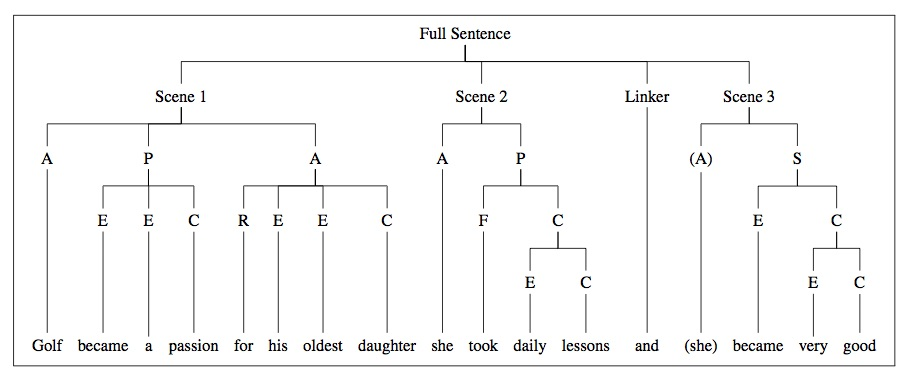
\includegraphics[width=1\textwidth]{ucca-tree}
    \caption{UCCA Tree with scenes}
    \label{ucca-tree}
\end{figure*}

%As you can see 
As can be seen
in Figure~\ref{ucca-tree}, the UCCA annotation results in a tree structure where each leaf is linked to
a word in the sentence at the bottom. A scene must contain a process (P) or a state (S). It can also contain
participants (A) and it can be linked to other scenes by a linker (Linker). Participants, processes and states can be
further analysed into elaborators (E), centres (C) and relators (R). These labels are very 
%high level 
high-level 
and relate to
cognitive concepts which should remain stable across languages.  

The fact that in UCCA
the labels are cognitive concepts and that they are linked directly to words
are both advantages 
when considering which semantic formalism is appropriate for machine translation evaluation.

One of such alternative formalisms is
Abstract Meaning Representation 
%%% Macro broken?
%(AMR; \inparcite{banarescu2013amr}). 
\cite{banarescu2013amr}. 
AMR is being actively developed with 
%the view to 
a view towards
using it as a way of generating 
translations but AMR graphs are not aligned to the words in the sentences. Having more abstract semantic structures 
makes the link between source words, target words, and structures more complex and potentially less useful. 
Furthermore, AMR  has been developed mainly with English in mind, and it remains
to be seen how universal AMR graphs are. See
\shortcite{amr:interlingua:lrec:2014} for first observations of divergences
between English 
%vs.
vs.\ 
Chinese and
Czech AMRs.

Another possible semantic framework for this kind of MT evaluation is Semantic
Role Labelling 
%(SRL; \inparcite{palmer2010semantic}).
\cite{palmer2010semantic}.
SRL has been used in a human translation metric called HMEANT~\cite{lo2011structured}. 
HMEANT uses semantic role labels
to measure how much of the “who, why, when,
where” has been preserved in translation. Annotators are instructed to identify verbs as
heads of semantic frames. Then they attach role
fillers to the heads and finally they align heads
and role fillers in the candidate translation with
those in a reference translation. Using SRL for evaluating SMT has a number of
disadvantages as explored by
\shortcite{birch-EtAl:2013:WMT} for German, \shortcite{bojar:wu:ssst:2012} for
Czech and by \shortcite{chuchunkov-tarelkin-galinskaya:2014:SSST-8} for Russian.
The most important drawbacks are as follows:
\begin{itemize}
\item SRL frames are based around a verb which is particularly problematic for
copular verbs and  when verbs are translated correctly as nouns or correctly
omitted (the verb ``to be'' in some Russian constructions).
\item SRL frames do not cover the entire source sentence and the semantic structure is
therefore not completely defined, importantly links between frames are not
considered and prepositional phrases which attach to nouns are not marked.
\item Even considering a limited set of eleven roles (agent, patient,
experiencer, locative etc.) is problematic because we cannot assume that these roles will 
 remain stable across different languages. 
 When looking at an automatically parsed  English-Chinese  parallel corpora,
 it was shown that 8.7\% of the arguments do not preserve their semantic roles~\cite{fung2006automatic}. 
\end{itemize}

UCCA provides universal semantic structures which 
%has 
have
a minimal set of labels. It provides a complete semantic tree which does not rely on syntactic heads and the semantic structure is grounded directly to the words in the sentence. 
 Even though the set of UCCA labels are fairly restricted,  nevertheless they allow us to determine the most important components of the graph (for example it defines centres and linkers which would be likely to carry more weight than elaborators), and we can use this to better calculate the score. 
We think that UCCA is the
most promising representation for evaluating translation. 

\subsection{Copied from emails}


UCCA-Eval in contrast to HMEANT:

- needs *very* trained UCCA annotators
- we were not very quick at explaining even the Eval annotations, but I guess we could have done better
+ relies only on one structure
+ relies on automatic alignment (in the form of hints only)
  These two positive design decisions are in line with what Dekai observed for HMEANT (see the abstract of http://repository.ust.hk/ir/Record/1783.1-66107): IAA of SRL drops from 90 to 61 when the two aligned structures are from two different annotators.

+ allows for multi-word and even non-contiguous elements
+ allows to indicate the quality of the predicates ("Actions")
+/- expects to cover the whole hypothesis with annotations, whereas HMEANT 'gives up' when the hypothesis is not intelligible, giving a zero score to the bad frame/whole sentence. This can be a good decision for HMEANT, since our way may artificially boost the chances of understanding the sentence.


HMEAN disadvantages:
. Importantly: it disregards copula clauses, nominalizations (which are often translated to verbal clauses), inter-clause relations (discourse markers, complement clauses etc.). UCCA-Eval addresses these.

Actually, I think this is a +/- . UCCA-Eval only needs the semantic evaluation done once for a given test source, whereas for the HMEANT set-up you have to keep annotating MT output. That's a + for UCCA-Eval. However we need bilingual annotators, which should be a -. Of course we could align translation and reference using monolingual annotators, but then we have the problem of alignment.
In the *MEANT papers they mainly test by either
A) correlating the metric to ranking judgements; or
B) using automated versions of the metric for tuning MT systems

I think neither is particularly convincing, but I'm not sure at the moment what we replace them with. Dekai also made a claim about the *MEANT metrics being "interpretable" in the sense that they could guide you towards semantic errors that the MT system may be making, however I don't recall seeing this done in his papers. 


By the claim that HMEANT explains things, Dekai probably means that the score is decomposable, but so is UCCA-Eval and even BLEU. And UCCA-Eval has one benefit over HMEANT: it points to words in the MT output that are aligned with something but do not convey the meaning well (and we know which part of the source meaning). Pure HMEANT might say only that some part of the MT output has no clear frames whatsover (and we do not know which part of the source/reference, unless we add the word alignments).




Differences of our approach:

The annotation experiment that we just conducted differs in two main ways from HMEANT:
1) The semantic framework is different - UCCA vs SRL - and SRL has problems which Omri lists below, some of which Dekai dismissed when they were brought up. Maybe these problems do not matter for MT evaluation or tuning, but I think this would have to be determined empirically.
2) The annotation process is different. We semantically annotate the source, then automatically project it to the translation, and ask bilingual annotators to assess whether this projection shows a good or bad translation. In HMEANT they semantically annotate both the reference and the translation, then align these manually, and assess to what extent they match.

Advatages of our approach:
Here is an additional argument to support the need for target-only intelligibility:
http://www.aclweb.org/anthology/W14-4005
see Table  3 and the text in Section 5.2.
The more frames can people annotate in the hypothesis, the better the hypothesis overall.



\subsection{MT Evaluation Overview}

The basic strategy for annotating the semantics of the machine translations is to step through the source sentence semantic 
components, looking at the translation via the word alignments, and marking on the source structure
%, 
which parts have 
been correctly translated.
There are two kinds of components: a word or basic semantic unit, and a structural component which contains one or more sub-components. 

\subsubsection{Lexical nodes}
Lexical nodes are usually comprised of individual words. They are the leaf nodes on the tree, the smallest 
%meaning bearing 
meaning-bearing
units of the tree.
Leaf nodes can be labelled as green (correct), orange (partially correct) and red (incorrect). 
The traffic light system makes the marking of the
lexical units as simple as possible.

\begin{itemize}
\item Green: The meaning of the word or phrase has been largely captured.
\item Orange: the essential meaning has been captured, but some part of the translation is wrong. This could often be due to the translated word having the wrong tense, or the wrong morphology. 
\item Red: The essential meaning of the unit has not been captured.
\end{itemize}


\subsubsection{Structural nodes}

Structural nodes contain other nodes which could be either lexical or structural nodes. 
These nodes are also called parent nodes and they can be labelled as ``Adequate'' or ``Bad''. 
What we are trying to gauge for structural nodes
%, 
is if the children of these nodes
relate to each other in the same way in the source sentence and in the translation. 
There are many ways that the relationship between the children might go wrong in translation:
\begin{itemize}
\item One of the child nodes is missing from the aligned translation. 
\item An extra word or phrase has been inserted into the aligned  translation.
\item The components of the translation are ordered differently 
%to 
from
the source.
\end{itemize}

If any of these changes have occurred and this damages the meaning of the aligned translation, then we mark the 
structural node as ``Bad''. 
However if the arrangement of the child nodes is essentially correct, except that one or
more of the child nodes has themselves been translated wrongly (and so is marked
orange or red), then the structural node should be 
annotated as ``Acceptable''.

\begin{figure*}[t]
    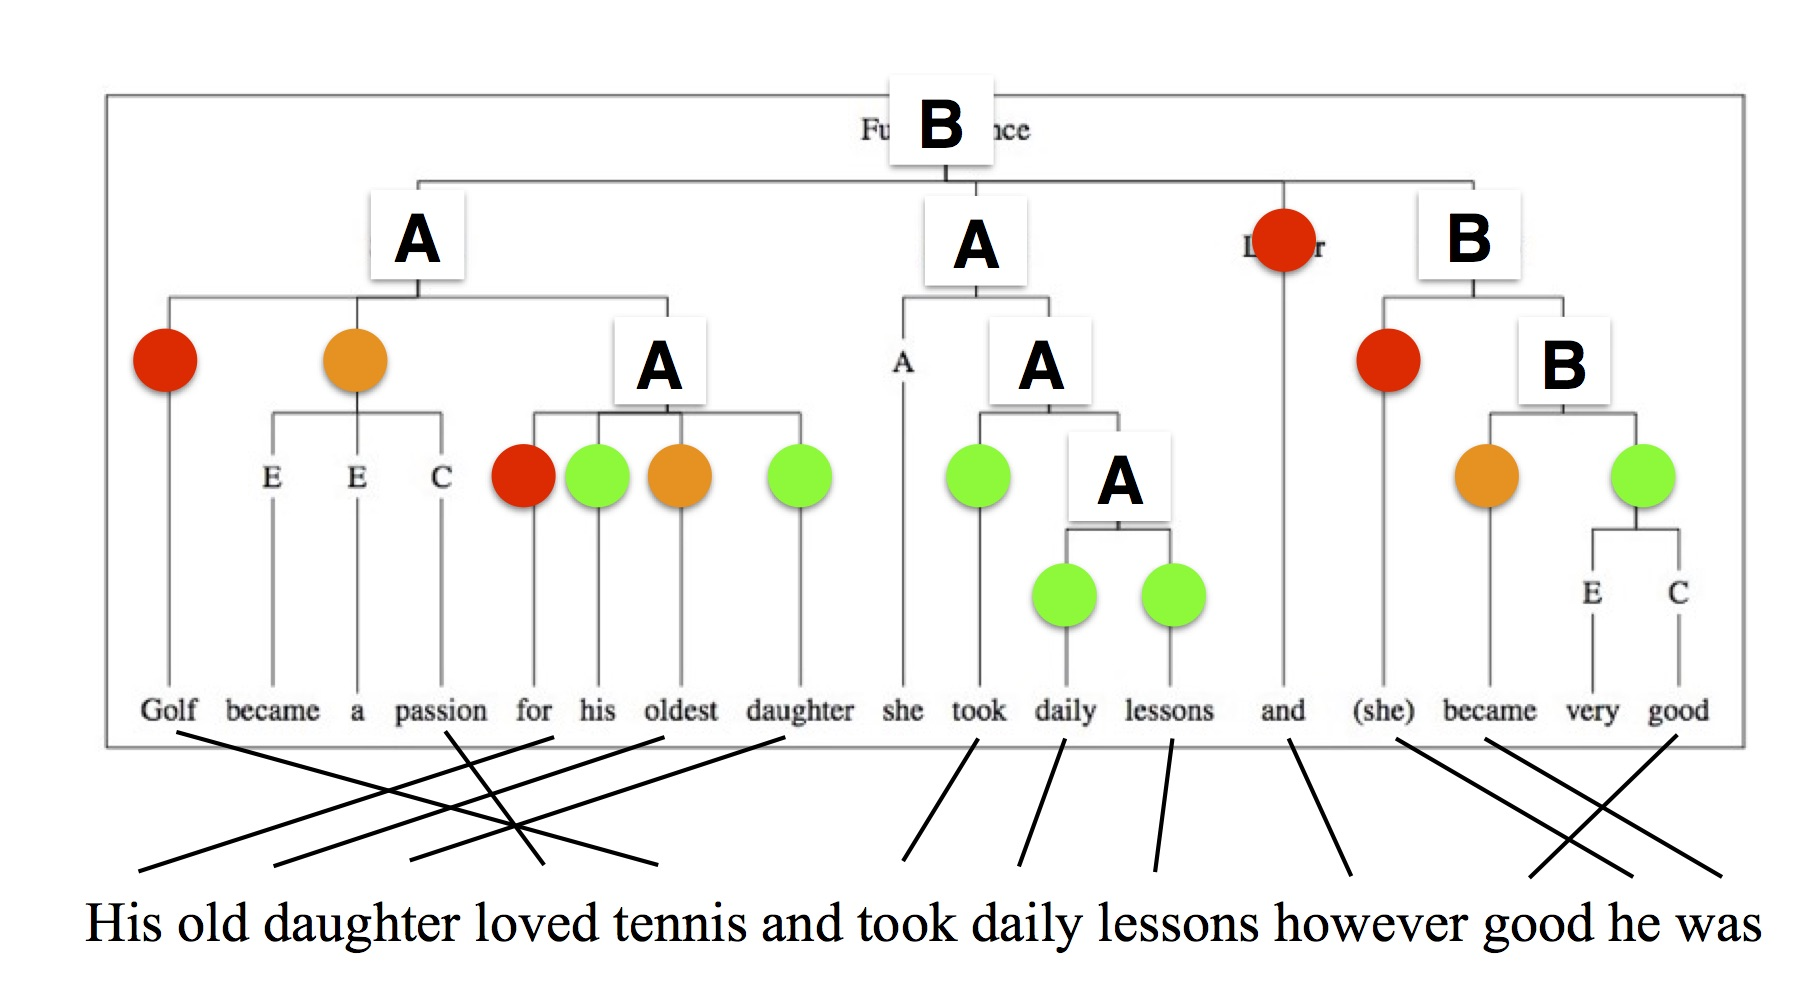
\includegraphics[width=1\textwidth]{ucca-tree-mteval}
    \caption{UCCA Tree evaluated in comparison to an aligned ``translation'' (an
	English paraphrase).}
    \label{ucca-tree-mteval}
\end{figure*}

%TODO describe figure 2 here

There are cases where we cannot usefully compare individual words in the source to words in the target.
We often need to compare translation at the phrase level. If this is the case, then we can 
 treat the structural node as a lexical unit, and mark it with the traffic light labels. This 
means that none of the children of this node will be examined in order determine the semantic score
for this sentence. 
In Figure~\ref{ucca-tree-mteval}, we can see that the phrase ``became a passion'' has been labelled as a lexical
node and it has been evaluated as ``Orange'', or partially correct, as the translation of this phrase ``loved'' 
only partially capture the semantics of the source.

We are separating lexical and structural evaluation in order to simplify evaluation and to localise errors
to their point of origin. For this reason, if a word has been translated incorrectly,
the parent node should still be correct if the number and relationship between its children are the same
as in the source. 
In Figure~\ref{ucca-tree-mteval}, we can see that even though an important child of the first scene is 
incorrectly translated (``Golf''), and the children of are ordered differently, 
the scene itself is marked as ``Acceptable''. The translation of the scene retains the structural 
relationships between the children.
\\

\newpage

\subsection{Machine Translation Evaluation Tool}

In this section, we will describe the tool that the annotators used to perform the annotation. 

\begin{figure*}[t]
    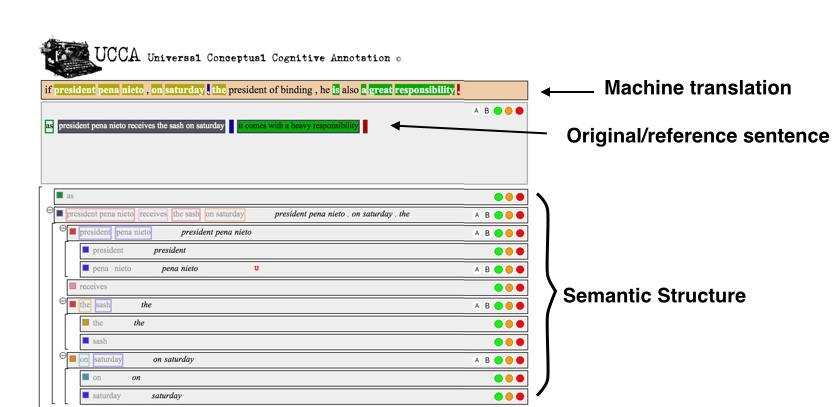
\includegraphics[width=1\textwidth]{interface-annotations}
    \caption{Machine translation evaluation tool}
    \label{mttool}
\end{figure*}

In Figure~\ref{mttool} you can see the MT evaluation tool. The sentence at the top shows the complete MT system output. Underneath the MT output is the  source sentence.  Underneath the source sentence we see its expandable semantic tree structure with both lexical and structural nodes. Lexical nodes only have traffic light annotation, whereas a structural node would normally be labelled ``A'' or ``B'' but could also be labelled as a lexical node, in the case where there is no word to word correspondence for the translation of its children.

 The child components of a structural node are marked with different coloured rectangles. When navigating through the different source sentence nodes, one can see the relevant sections of the translation because the aligned words in the translation are highlighted in the complete sentence above. Aligned translations are also shown in black alongside the source node. If the node is aligned to a set of discontiguous words in the translation, then the unaligned words that appear in between the aligned words are shown in red. Even if these words are not directly aligned to the source node, they 
will likely change the meaning of the translation and must be considered when marking 
the translation as correct or not. The alignments are meant just as a guide. The annotator should  look at the complete translation when deciding on the evaluation of a node. The translation could have content added before or after the node which changes its
 structure or meaning. If an extra component is prepended to a structural node, for example, it should be marked as ``Bad''.

%\subsection{Example}
%
%\lexi{TODO write this up}
%
%NODE1. (make sure) (you’ve got a solid chair)
%MT: (stellen Sie sicher, dass) (Sie haben einen festen Stuhl)
%Correct would be: (stellen Sie sicher, dass) (Sie einen festen Stuhl haben)
% 
%NODE2. (you) (’ve) (got) (a solid chair)
%MT: (Sie) (haben) (einen festen Stuhl)
%Correct would be: (Sie) (einen festen Stuhl) (haben)
%
%Node 1 is the parent node of Node 2. The error in MT is that the verb in German "haben" appears in the wrong place, it should be at the end and this makes the translation difficult to understand. The place to mark this error is where haben is a child node, ie. the error occurs in Node 2. This is where the relationship or the order between the child nodes (Sie)(haben) and (einen festen Stuhl) is wrong. The error propagates up to Node 1, but at Node 1 we are evaluating the relationship between (stellen Sie sicher, dass) and (Sie haben einen festen Stuhl) and this is correct and should be marked A. 

\newpage



\subsection{Results}

%new_mteval_ro1: Christian
%new_mteval_ro2: Rodica  NHS
%new_mteval_pl1: Malgorzata
%new_mteval_pl2: Iwona (starting from the 29th in the sequence) NHS
%new_mteval_cs1: Martina
%new_mteval_de1: Juliane (starting from the 28th in the sequence)

In this section we report the results of the evaluation. We first report some statistics which give us an overall idea
of how the annotators fared. We then delve into the question of how reliable the annotations are by examining
inter-annotator agreement and looking at confusion matrices. Finally we calculate UCCA semantic scores
for the different language pairs.  

\subsubsection{Overall Statistics}

In order to explore the results of our annotations, we first show some basic statistics
about the task. In Table~\ref{tab:stat-all}, we can see the total number of sentences annotated
%
with
the number of nodes. We also show the percentages of the main types of nodes.
Looking at this table we see that the number of sentences varies from 324 to 351 sentences,
except for Ro1 who did considerably fewer, only 230. 
All annotators were shown the same set of sentences, but their results were only
collected if they pressed the submit button. So these missing sentences were either mistakenly
not submitted, or they did not get to the end of the task. 
Looking at the types of nodes annotated, these seem to be distributed quite uniformly.
About 35\% of the nodes were considered to be structural, and 60\% to be lexical.
Some nodes were not evaluated, and these are called ``Missing''. 
The node may represent an English
word which is not required in the target language (often an article or a
pronoun).
As per instructions, the annotators were expected to mark such nodes with green
but some may have left the node unannotated (in which case it would be perhaps
appropriate to consider the parent as a lexical node).
With hindsight, we should have introduced a separate annotation category for this, and
also enforced the lexical/structural distinction in the tool. ``Missing''
annotations are not very common, but
one annotator left 6.2\% of the nodes unlabelled which is a bit too high and in 
future experiments we will alter the tool to disallow missing nodes, unless their parent is a lexical node. 

\begin{table}[h!]
\begin{center}
      \begin{tabular}{|l|c|c|c|c|c|}
      \hline
 & \bf{No. Sentences} & \bf{No. Nodes} & \bf{\%Structural} & \bf{\%Lexical}  & \bf{\%Missing} \\
\hline                               
    De1  &  339 &  9253 & 36.2 & 62.5 & 1.3 \\ 
    Cs1  & 324 &  8794 & 33.4 & 63.3 & 3.3\\ 
    Ro1  & 230 &  6152 & 36.4 & 62.7 & 0.8\\ 
    Ro2  & 337 &  9228 & 35.6 & 61.4 & 2.9 \\ 
    Pl1  & 351 &  9557 & 34.0 & 59.8 & 6.2 \\ 
    Pl2  & 340 &  9303 & 31.0 & 64.6 & 4.4 \\ 
      \hline
    \end{tabular}
\end{center}
\normalsize
\vspace*{-3ex}
\caption{Number of annotated sentences and nodes and the percentages of each of the main kind of nodes
}
\label{tab:stat-all}
\end{table}

\begin{table}[h!]
\begin{center}
      \begin{tabular}{|l|c|c|c|}
      \hline
   & \bf{No. Nodes} & \bf{\%A} & \bf{\%B}   \\
\hline                               
    De1  &  3350 &  68.2 & 31.7  \\ 
    Cs1  & 2939 &  73.4 & 26.6 \\ 
    Ro1  & 2239 &  68.2 & 31.8  \\ 
    Ro2  & 3286 &  65.4 & 34.6 \\ 
    Pl1  & 3246 &  50.3 & 49.7 \\ 
    Pl2  & 2884 &  71.5 & 28.5 \\ 
      \hline
    \end{tabular}
\end{center}
\normalsize
\vspace*{-3ex}
\caption{Number of structural  nodes and the percentages of each of the types of nodes
}
\label{tab:stat-struct}
\end{table}

In Table~\ref{tab:stat-struct}, we can see the number of structural nodes, and their
breakdown in terms of acceptable  ``A'' or bad ``B''. Most annotators seem to 
label about 70\% of the structural nodes as correct. The exception is Pl1 who
seems to be following a different annotation strategy. It is possible that Pl1 
did not understand the guidelines correctly. Further investigation with a Polish
speaking colleague will be necessary.

\begin{table}[h!]
\begin{center}
      \begin{tabular}{|l|c|c|c|c|}
      \hline
   & \bf{No. Nodes} & \bf{\%G} & \bf{\%O}  & \bf{\%R} \\
\hline                               
    De1  & 5784  &  70.8 & 13.0 & 26.6  \\ 
    Cs1  & 5568 &  62.8 & 18.4 & 18.8 \\ 
    Ro1  & 3859 &  75.9 & 8.4 & 15.7  \\ 
    Ro2  & 5671 &  68.7 & 16.9 & 14.3 \\ 
    Pl1  & 5717 &  60.8 & 13.1 & 26.1 \\ 
    Pl2  & 6007 &  49.6  & 17.3 & 33.0 \\ 
      \hline
    \end{tabular}
\end{center}
\normalsize
\vspace*{-3ex}
\caption{Number of lexical  nodes and the percentages of each of the types of nodes
}
\label{tab:stat-lex}
\end{table}

In Table~\ref{tab:stat-lex} we can see the number of lexical nodes, and their
breakdown in terms of correct  ``G'', partial ``O'' or incorrect ``R''. 
There is more variation here between the annotators than for the
structural nodes. The percentage of correct nodes fluctuates from 49.6\%
to 75.9\%. One expects that  languages with different amounts of 
morphology and agglutination would report different numbers here,
but even amongst annotators of the same languages the results vary.
For Polish the number of correct lexical 
%node 
nodes
varies between 49.6\%
and 60.8\%.

\subsubsection{IAA}

In order to determine how reliable our human evaluation approach is, we need to
examine the agreement that we find between annotators.
For two of the language pairs, Romanian and Polish, we had 2 annotators. 
 Inter-annotator agreement can be calculated 
using the Kappa score which is more reliable than agreement because it takes into
account the probability of agreement by chance. 

%Lexi TODO put Kappas in a separate table

\begin{table}[h!]
\begin{center}
      \begin{tabular}{|l|cc|c|}
      \hline
\bf{MT Eval Label} & \bf{A} & \bf{B} & \bf{All} \\
\hline                               
    A   & 1096 &  285 & 1381\\ 
   B   & 101 & 507  & 608\\ 
   \hline
   All &  1197 &  792 & 1989\\
      \hline
    \end{tabular}
\end{center}
\normalsize
\vspace*{-3ex}
\caption{Confusion Matrix for the structural nodes for the Romanian annotators with a Kappa of 0.58
}
\label{tab:iaa-ab-ro}
\end{table}

\begin{table}[h!]
\begin{center}
      \begin{tabular}{|l|ccc|c|}
      \hline
\bf{MT Eval Label} & \bf{R} & \bf{O} & \bf{G} & \bf{All} \\
\hline                               
   R   & 2274 &  361 & 126 & 2761 \\ 
   O   & 92 & 164  & 37 & 293 \\ 
   G   & 82 & 76  & 358 & 516 \\ 
   \hline
   All &  2448 &  601 & 521 & 3570\\
      \hline
    \end{tabular}
\end{center}
\normalsize
\vspace*{-3ex}
\caption{Confusion Matrix for the lexical nodes for the Romanian annotators with a Kappa of 0.50
}
\label{tab:iaa-rgo-ro}
\end{table}

In Tables~\ref{tab:iaa-ab-ro} and \ref{tab:iaa-rgo-ro} we see the confusion matrix of
the two main types of evaluation labels for Romanian. We separate structural and lexical nodes, because
there is very little disagreement between annotators about which node is a lexical and which
node is structural, and so if we calculate Kappa over all the values, this might artifically 
inflate our IAA scores.
For both structural and lexical nodes, the Kappa values 
of 0.58 and 0.50 respectively 
can
be considered to display moderate agreement. 
If we calculate Kappa scores across all five categories, it rises to 
0.69 because of the strong agreement about what is a lexical and a structural 
node. 


%\lexi{TODO look at confusion between structural and lexical}

\begin{table}[h!]
\begin{center}
      \begin{tabular}{|l|cc|c|}
      \hline
\bf{MT Eval Label} & \bf{A} & \bf{B} & \bf{All} \\
\hline                               
    A   & 1208 &  192 & 1400 \\ 
   B   & 681 & 574  & 1255 \\ 
   \hline
   All &  1889 &  766 & 2655 \\
      \hline
    \end{tabular}
\end{center}
\normalsize
\vspace*{-3ex}
\caption{Confusion Matrix for the structural nodes for the Polish annotators with a Kappa of 0.33
}
\label{tab:iaa-ab-pl}
\end{table}

\begin{table}[h!]
\begin{center}
      \begin{tabular}{|l|ccc|c|}
      \hline
\bf{MT Eval Label} & \bf{R} & \bf{O} & \bf{G} & \bf{All} \\
\hline                               
   R   & 2430 &  444 & 427 & 3301 \\ 
   O   & 119 & 398  & 198 & 715 \\ 
   G   & 161 & 109  & 1110 & 1380 \\ 
   \hline
   All &  2710 &  951 & 1735 & 5396 \\
      \hline
    \end{tabular}
\end{center}
\normalsize
\vspace*{-3ex}
\caption{Confusion Matrix for the lexical nodes for the Polish annotators with a Kappa of 0.58
}
\label{tab:iaa-rgo-pl}
\end{table}

In Tables~\ref{tab:iaa-ab-pl} and \ref{tab:iaa-rgo-pl} we see the confusion matrix of
the two main types of evaluation labels for Polish. Here we see similar Kappa results for
the lexical nodes (0.56) but the Kappa for structural nodes drops to 0.33. 
This low agreement could be the result of one annotator misinterpreting the guidelines
and warrants further analysis.
If we calculate Kappa scores across all five categories, it rises to 
0.58. 

Looking beyond Kappa scores, we did some analysis of the cases where
one annotator marked a word as Red and another marked it Green. 
For Polish  the most common English words about which the annotators
disagreed were: ``to'', ``you'', ``blood'' (which was aligned to ``krwi''), ``in'' and ``for''. 
For Romanian, the words were ``you'', ``to'', ``the'', and ``your''. 
Apart from ``blood'', all these words are short function words which can 
be translated in a very different fashion in the target and this could contribute to
 confusion about
whether they are correct or not.

Looking at the words which were marked Red most often again these were largely function words.
This is partially due to the fact that they occur more frequently than other words. But
words such as ``bias'', ``falls'', ``fibrillation'' and ``review'' also occur frequently in this list and these
are words with domain specific translations which we are possibly not capturing with
the unadapted HimL models.

\subsubsection{UCCA Scores}

\paragraph{Node score} This simple score reflects the percentage of correct MT evaluation nodes. 
A and G are correct, O counts as 50\% correct and R and B count as incorrect. Nodes which are missing an
evaluation are ignored.

\begin{table}[h!]
\begin{center}
      \begin{tabular}{|l|c|c|c|}
      \hline
\bf{Annotator ID}  & \bf{Structural } & \bf{Lexical } & \bf{Overall }\\
\hline                               
    De1  &  68.20 & 77.40 & 74.03 \\ 
    Cs1  & 73.35 & 72.00 & 72.46 \\ 
    Ro1  & 68.15 & 80.09 & 75.71 \\ 
    Ro2  & 65.42 & 77.26  & 72.92 \\ 
    Pl1  & 50.33 & 67.33 & 61.17 \\ 
    Pl2  & 71.53 &58.26  & 62.56 \\ 
      \hline
    \end{tabular}
\end{center}
\normalsize
\vspace*{-3ex}
\caption{Node scores: percentage of correct nodes. 
}
\label{tab:node_scores}
\end{table}

In Table~\ref{tab:node_scores} we can see the simple node scores for the different annotators. 
Results show that most systems are evaluated as having about 70\% correct overall, with the
notable exception of both Polish annotators. They gave scores to the HimL test set which
were about 10\% lower. English$\to$Polish is considered to be a very challenging language pair
for machine translation and so this result is not surprising.  Another trend is that the annotators gave the lexical scores of at least 
10\% higher than the structural scores for three out of five annotators. The two remaining
annotators behaved quite differently. Cs1 gave similar scores for structural and lexical nodes, but
Pl2 gave much better scores for structural nodes (71.53 vs. 58.26). 
The differences in behaviour displayed by the two Polish annotators in this table and the
low kappa reported in Table~\ref{tab:iaa-ab-pl}
brings into question the reliability of the Polish annotations.  


\begin{figure*}[t]
    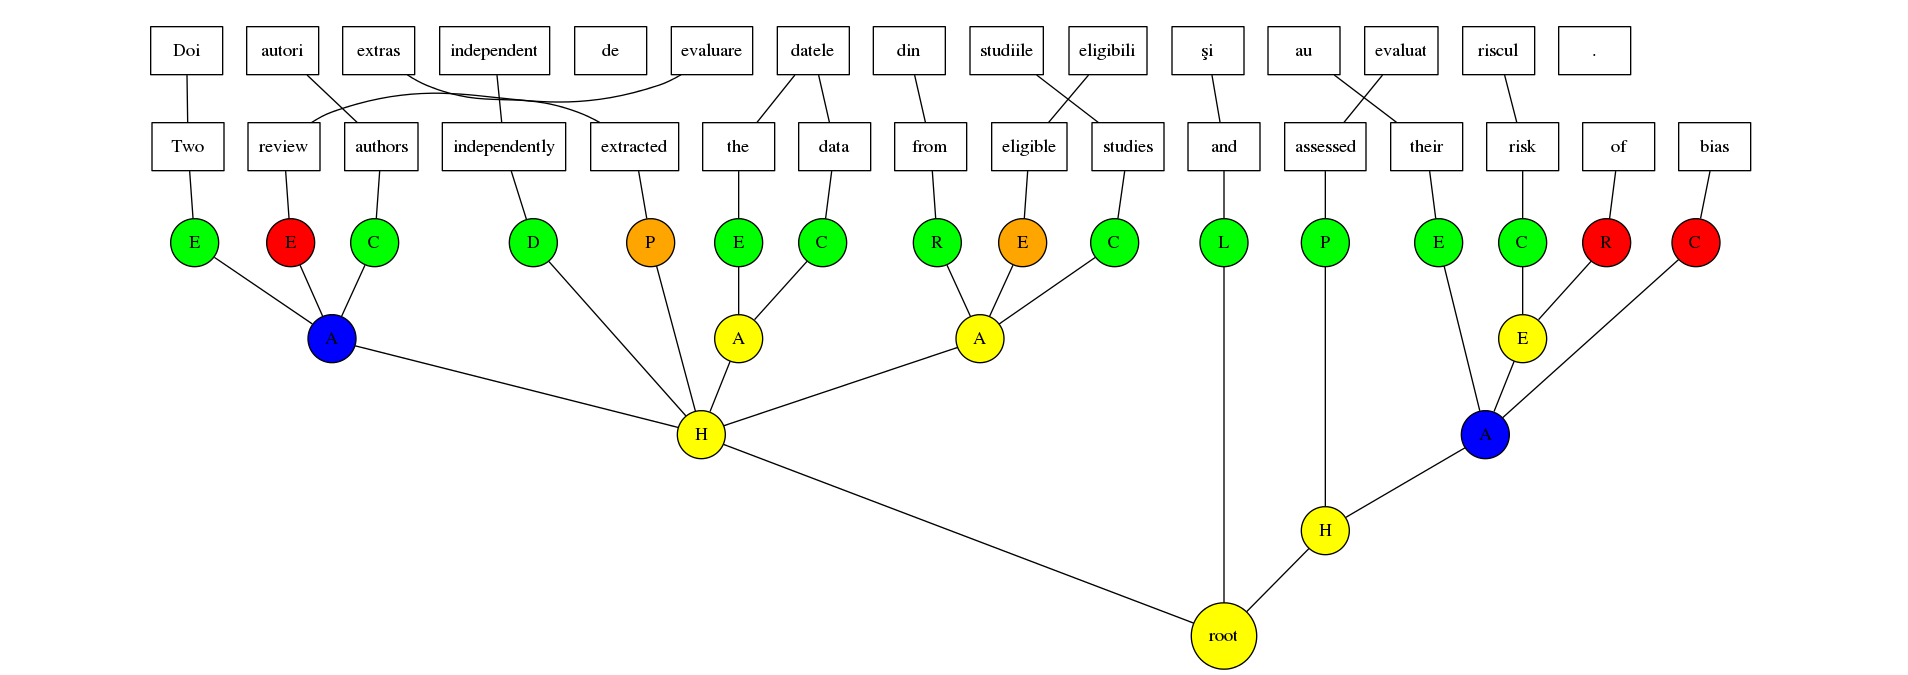
\includegraphics[width=1.1\textwidth]{tree_convert.png}
    \caption{UCCA tree on the source labelled with the MT Eval labels and aligned to the target translation. The 
    ``Acceptable'' structural nodes are yellow, the ``Bad'' ones are blue.}
    \label{fig:ucca-tree-evaluated}
\end{figure*}

%\lexi{TODO: Any chance of an example with bad structural nodes ? }
In order to visualise the UCCA evaluation results and see how the node scores are calculated, we provide an  example from the experiment. 
Looking at Figure~\ref{fig:ucca-tree-evaluated}, we can see the machine translation at the top. Below this are the word alignments to the English source. 
Each of the English words (except punctuation) are linked to UCCA lexical nodes which have been evaluated as either
correct (green), partially correct (orange) or incorrect (red). The letters inside the circles correspond to the UCCA node types
which will be important in future versions of the score. Structural nodes are either acceptable (yellow) or bad (blue). 
So for this sentence given that we have 11 green nodes, 2 orange nodes, 6 yellow nodes and in total there are 24 nodes:

\begin{displaymath}
node score = \frac{ 11  + 0.5 ( 2 ) + 6  } { 24  } * 100\\
                    = 75
\end{displaymath}

\subsection{Discussion}

In this evaluation we have proposed an evaluation which has a number of advantages:
\begin{itemize}
\item  It shows moderate IAA agreement which means that our metric is relatively reliable. It is not directly comparable to other metrics because HMEANT papers do not report IAA and they had to rely on agreement statistics which can be misleading. 
\item  We can reuse the UCCA structures on the source multiple times, and as this is the most time consuming part
of the evaluation, this makes best use of expensive expert annotators. 
\item Translation annotators do not have to try to create semantic structures on erroneous machine translation output, in fact
they do not need to create any semantic structures at all as this can be done previously by experts.
\item Errors are isolated at the point where they occur due to the separation of structure and lexical content and there
is little ambiguity about whether an error in a leaf needs to be counted multiple times as we go up the tree. 
\item UCCA provides a minimal yet complete semantic framework which is based on universal cognitive concepts. 
The structure does not rely on syntactic heads and the semantic graph is grounded directly to the words in the sentence. 
\end{itemize}

The evaluation also brought up a number of issues that will need to be resolved by either better  training or
by improving the tool. Many of these issues were reported by the annotators:
\begin{itemize}
\item Isolating errors to the point where they occur is difficult to do for humans as there is a tendency to
penalise the parent nodes for errors which occur in their children. 
\item Initially some annotators struggled to understand the distinction between lexical and structural nodes. 
\item They also had some difficulty evaluating the 
%sentence 
sentences
without their context. 
\item The annotators were unsure about how to judge incorrect morphology or tense. 
\item  The alignments were meant only as a guide and some words are unaligned or doubly aligned and this
caused some confusion. 
\item Extraneous additions on the target might not be penalised unless they fall inside the source
semantic structure.
\end{itemize}

Even though there have been a number of issues which have arisen, the UCCA evaluation has shown to be a reliable and
efficient
method for evaluating the accuracy of HimL translation systems. 
We will continue to analyse the results from this experiment and we will run an improved version of
 this evaluation in year two
of the project. 

%Comments from Juliane (Cochrane DE)
%- There weren't many, but a few mistakes in the source, that made it difficult to annotate.
%- Sometimes it was difficult to judge without context, but not very often - at least if you're familiar with the content.  
%- There were cases where the way the sentences were segmented made it difficult to annoate them in a useful way.
%- Many wrong declinations and conjugations.
%- German genus requires pronouns or articles to be repeated in lists of nouns in order to be correct, e.g. your strength and balance = Ihre Stärke und Ihr Gleichgewicht
%- There were a few out of domain vocabulary instance, e.g. "balance" being translated in the context of banking rather than the body, but only in one or two sentences, not in all where it occured. Similarly, the word "trial" got translated as "process", "study", and in the context of a court trial. 
%- A number of Cochrane or medical research specific terms was not well translated.
%- Abbreviations never got translated correctly.
%- Participle constructions often mess up the translation completely.
%- Some verbs kept getting translated as nouns or the other way round, e.g. in review author = the author of a review, review was always interpreted as a verb; falls (noun) was mostly translated as verb. 
%- Overall: both Cochrane and NHS sentences were more often bad than understandable. Only very few were acceptable for publication on our websites in my view. I guess that was expected :)
%What I mentioned earlier:
%- The past and future tense were often ignored, which is usally not a problem for future, but for past it is
%- Fairly often verbs were not translated at all (e.g. "cause" was never translated).  
%- If the verb is present, it is often in the wrong order with the subject, as it doesn't necessarily follow the same order as in English.
%- You is sometimes translated formally and sometimes informally, even in the same sentence.
%- Need a counter to know how many sentences completed
%
%Comments from Rodica (NHS Ro):
%One of the most recurrent confusions I had during my work was in connection with the word order in the MT.
%EG.  English: This review provides limited evidence that interventions...
%         Romanian: Acest studiu intervenții care furnizează dovezi limitate
%                               (This review interventions provide limited evidence)
%My question would have been how to mark the wrong or random word order in the MT translation, when the individual words appeared, so they couldn't be marked as red. 
%In most of the examples this occurred in the Romanian translations  because the default word order in Romanian is  noun + descriptive adjective(s), rather than the other way round and so, in the MT the descriptive adjectives would be first and sometimes other words would be added before the noun, which would make the sentence incomprehensible in Romanian.
%I think I mentioned to you the other questions during the work. The one that I should have asked earlier  was how far up the structure I should  mark a missing child. I understood it only once I spoke to you, but that was quite late.
%
%
%Comments from Iwona (NHS Polish)
%- Need a counter to know how many sentences completed
%1. Phrases split in wrong places, e.g. ‘depending on’, ‘there is’
%2. Certain phrases should be treated as one unit, e.g. ‘make sure’, so a leaf node for 
%marking as green, orange or red.
%3. Different sentence structure in English and Polish, e.g.
%‘our appetites often decrease’
%Machine translation: ‘our appetites often a fall’
%Correct translation:  ‘Often decreases for us appetite’
%Please note in the example above the meaning can be worked out and for that 
%reason I marked the structural node as A. However, this is bad Polish. There were a 
%number of sentences like this one, the translation of some of them made more sense 
%than others, on the whole it was difficult to annotate them. 
%4. The following is a common occurrence:
%‘before starting a new exercise programme’
%‘before’ – ‘przed rozpoczęciem’ (should be ‘przed’)
%‘starting’ – ‘przed rozpoczęciem’ (should be ‘rozpoczęciem’)
%Both leaf nodes have the same translation, but the translation appears only once in 
%the structural node. I marked the parent node as A, and the two leaf nodes as red. 
%5. Double negation in Polish causes problems at the structural level.


\subsection{Automatic Semantic Evaluation}

The results that we have gathered in this evaluation will be used as gold data to evaluate the performance of a number of automatic
metrics, to determine which of the existing metrics are most suited to evaluating accuracy.  We have also  initiated
work on developing an automatic version of the UCCA human evaluation task. For this we need an UCCA semantic parser
and data to train it, as the UCCA treebank is relatively small. We are looking at extracting further training examples from
the Prague treebank t-layer. This will be described in Deliverable D5.3, due at the end of July 2016. 


\section{Conclusion}

\section*{Acknowledgments}

Do not number the acknowledgment section.
This section should not be presented for the submission version.

\bibliography{main}
\bibliographystyle{acl2016}


\end{document}
